For the second iteration was the goal to remove the raycasting thats happens on runtime.

\subsection*{Minimizing the Graph size}
It was possible to reduce the number of waypoints even further.
To do so all waypoints are looped through to find adjacent waypoints, meaning waypoints whose distance to each other is less or equal to one.
Those that are adjacent are then removed and a new waypoint is placed halfway between them.
This is illustrated in Figure \ref{waypointMerge}.
The resulting waypoints can be seen in Figure \ref{waypointOpt} with the graph in Figure \ref{waypointgraphOpt}.
Most notably, the amount of edges are significantly reduced.
\begin{figure}[H]
	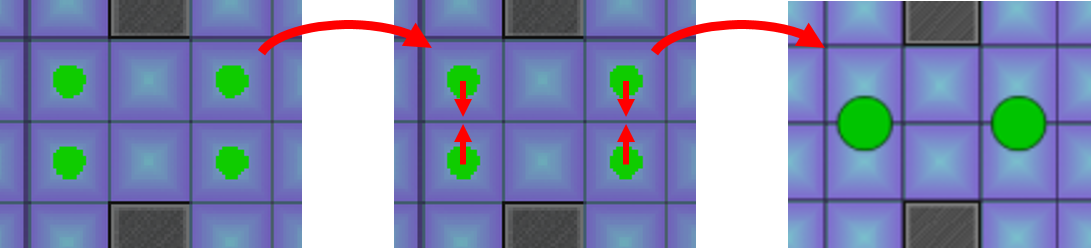
\includegraphics[width=\textwidth]{figures/astar/waypointMerge}
	\caption{Waypoint merging}
	\label{waypointMerge}
\end{figure}

\begin{figure}[H]
	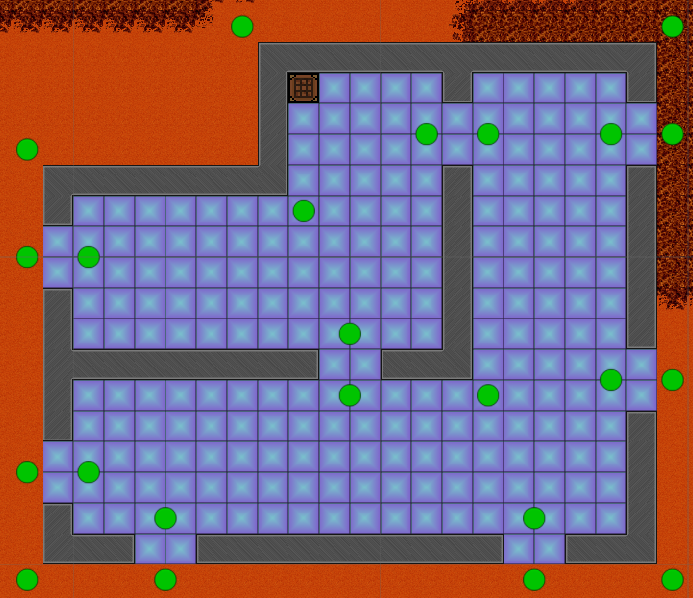
\includegraphics[width=\textwidth]{figures/astar/optimizedWaypoints}
	\caption{Waypoints after optimizations}
	\label{waypointOpt}
\end{figure}

\begin{figure}[H]
	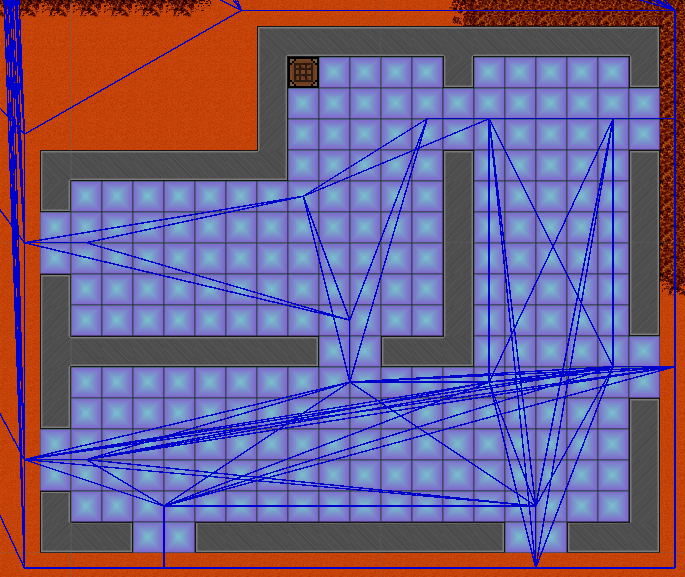
\includegraphics[width=\textwidth]{figures/astar/optimizedWaypointsGraph}
	\caption{Graph based on the waypoints after waypoint optimization}
	\label{waypointgraphOpt}
\end{figure}

\subsection*{Eliminating raycasts}
Raycast, in our case, is used to test if another object is accessible in a straight line.
This happens in two places:
\begin{itemize}
\item Enemies check to players
\item Enemies check to waypoints
\end{itemize}
The raycast from an enemy to a player happens when the enemy want to check if the player is accessible in a straight line.
To prevent the raycast check to the players the map is partitioned into convex rectangles.
When an enemy then enters the same partition as a player it knows that i can walk directly towards the player since the rectangle is convex.
Such partitions are generated while also generating the backdrop.
Rectangles are found using the same algorithm for finding rectangles for tiles. 
For finding rectangles for partitions an inverted version of the map representing collidable walls is used. 
The result of running the algorithm for finding the rectangles for partitions is illustrated in Figure~\ref{fig:partition_colliders_on_map}.

\begin{figure}[H]
        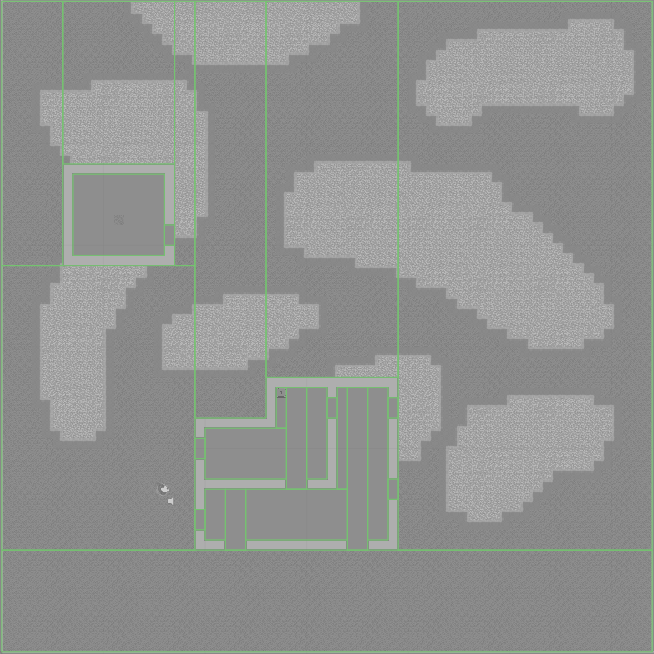
\includegraphics[width=0.9\textwidth]{figures/generating_levels/partition_colliders.png}
    \caption{Rectangles for partitions}\label{fig:partition_colliders_on_map}
\end{figure}

Once the partitions are made, trigger colliders are added to them.
These trigger colliders are used to add and remove a reference to partitions that enemies' and players' enters when they enters the region.
A list of partitions on the player and enemies is needed since their colliders can overlap with multiple partitions.

First optimisation is to check whether the player is in the same partition as the enemy and if so the enemy can go straight towards the player and the enemy will be in hunting mode.
Hunting mode means the enemy can afterwards check the neighbouring partitions once the player runs out of the partition.
The hunting mode prevents odd behaviour from the enemies when they runs after a players, since if there was no hunting mode the enemy would have to start pathfinding if a player leaves a the partition, as illustrated in Figure \ref{huntingMode}.

\begin{figure}[H]
        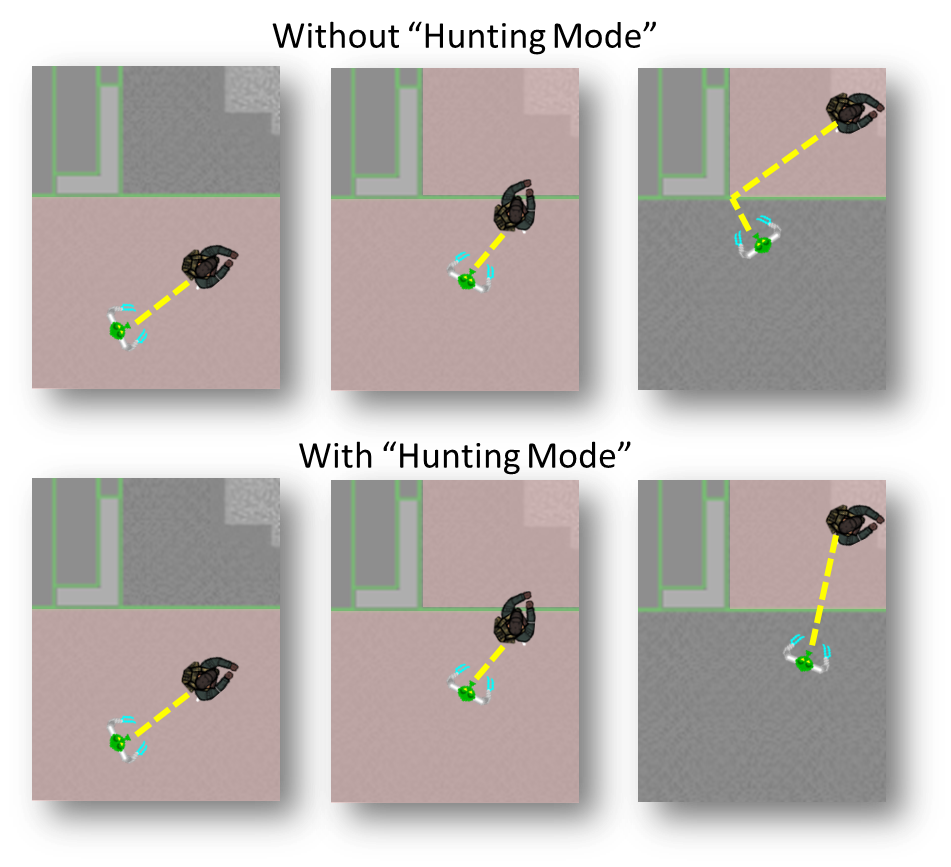
\includegraphics[width=\textwidth]{figures/astar/huntingMode.png}
    \caption{Behaviour difference between hunting mode and no hunting mode, showing if the players leave a partition the enemy without hunting mode would have to start pathfinding resulting in odd behaviour}\label{huntingMode}
\end{figure}

If the player then escapes, meaning that the player is not in the same partition nor in the neighbouring partitions the enemy will then start to run the pathfinding algorithm and follow the path until we have the player in sight again or reached the end of the path where we then have to run the algorithm again.

To eliminate the costly raycast happening when finding the nearest waypoints.

Therefore, we moved the pathfinding to load time where it finds the shortest path for all the possible paths, and saves it in a hashtable.
This means that when a enemy cannot see the player, it checks the table for possible path and then simply follows it.

